\section{Components and Bring-Up Changes}
\label{sec:hw-bom}

The fitted components are listed in \Cref{tab:hw-bom-provenance}. The board photographs show the resonant-branch changes made during bring-up.

\begin{table}[H]
\centering
\caption{Main components fitted to the prototype.}
\label{tab:hw-bom-provenance}
\small
\begin{tabularx}{\textwidth}{@{}p{0.25\textwidth}p{0.34\textwidth}X@{}}
\toprule
Function & Part & Value or function\\
\midrule
Input fuse & 04653.15DR & \SI{3.15}{\ampere}, \SI{250}{\volt} AC\\
Varistor & ERZV07D471 & Surge clamping\\
Input choke & 7448680200 & Two \SI{120}{\micro\henry} windings on V1.0\\
Pump capacitor & C1206X202FBGACTU & \SI{2}{\nano\farad}, \SI{630}{\volt}\\
DC-link capacitor & 860241478004 & \SI{22}{\micro\farad}, \SI{450}{\volt} fitted to the prototype\\
Pump diodes & PU1JLWH & Ultrafast steering rectifiers\\
GaN stage & LMG2652RFBR & Integrated half bridge and drivers\\
Final resonant branch & Two 7443640470B & \SI{9.4}{\micro\henry} nominal series total\\
Controller & STM32G071RBT6 & Carrier, enable timing, ADC DMA, and UART\\
Isolated voltage sensing & AMC0330 & Secondary-bulk feedback\\
Output stage & MPQ4242GVE-0000-AEC1-P & USB-C PD voltage regulation and interface\\
\bottomrule
\end{tabularx}
\end{table}

\begin{figure}[htbp]
\centering
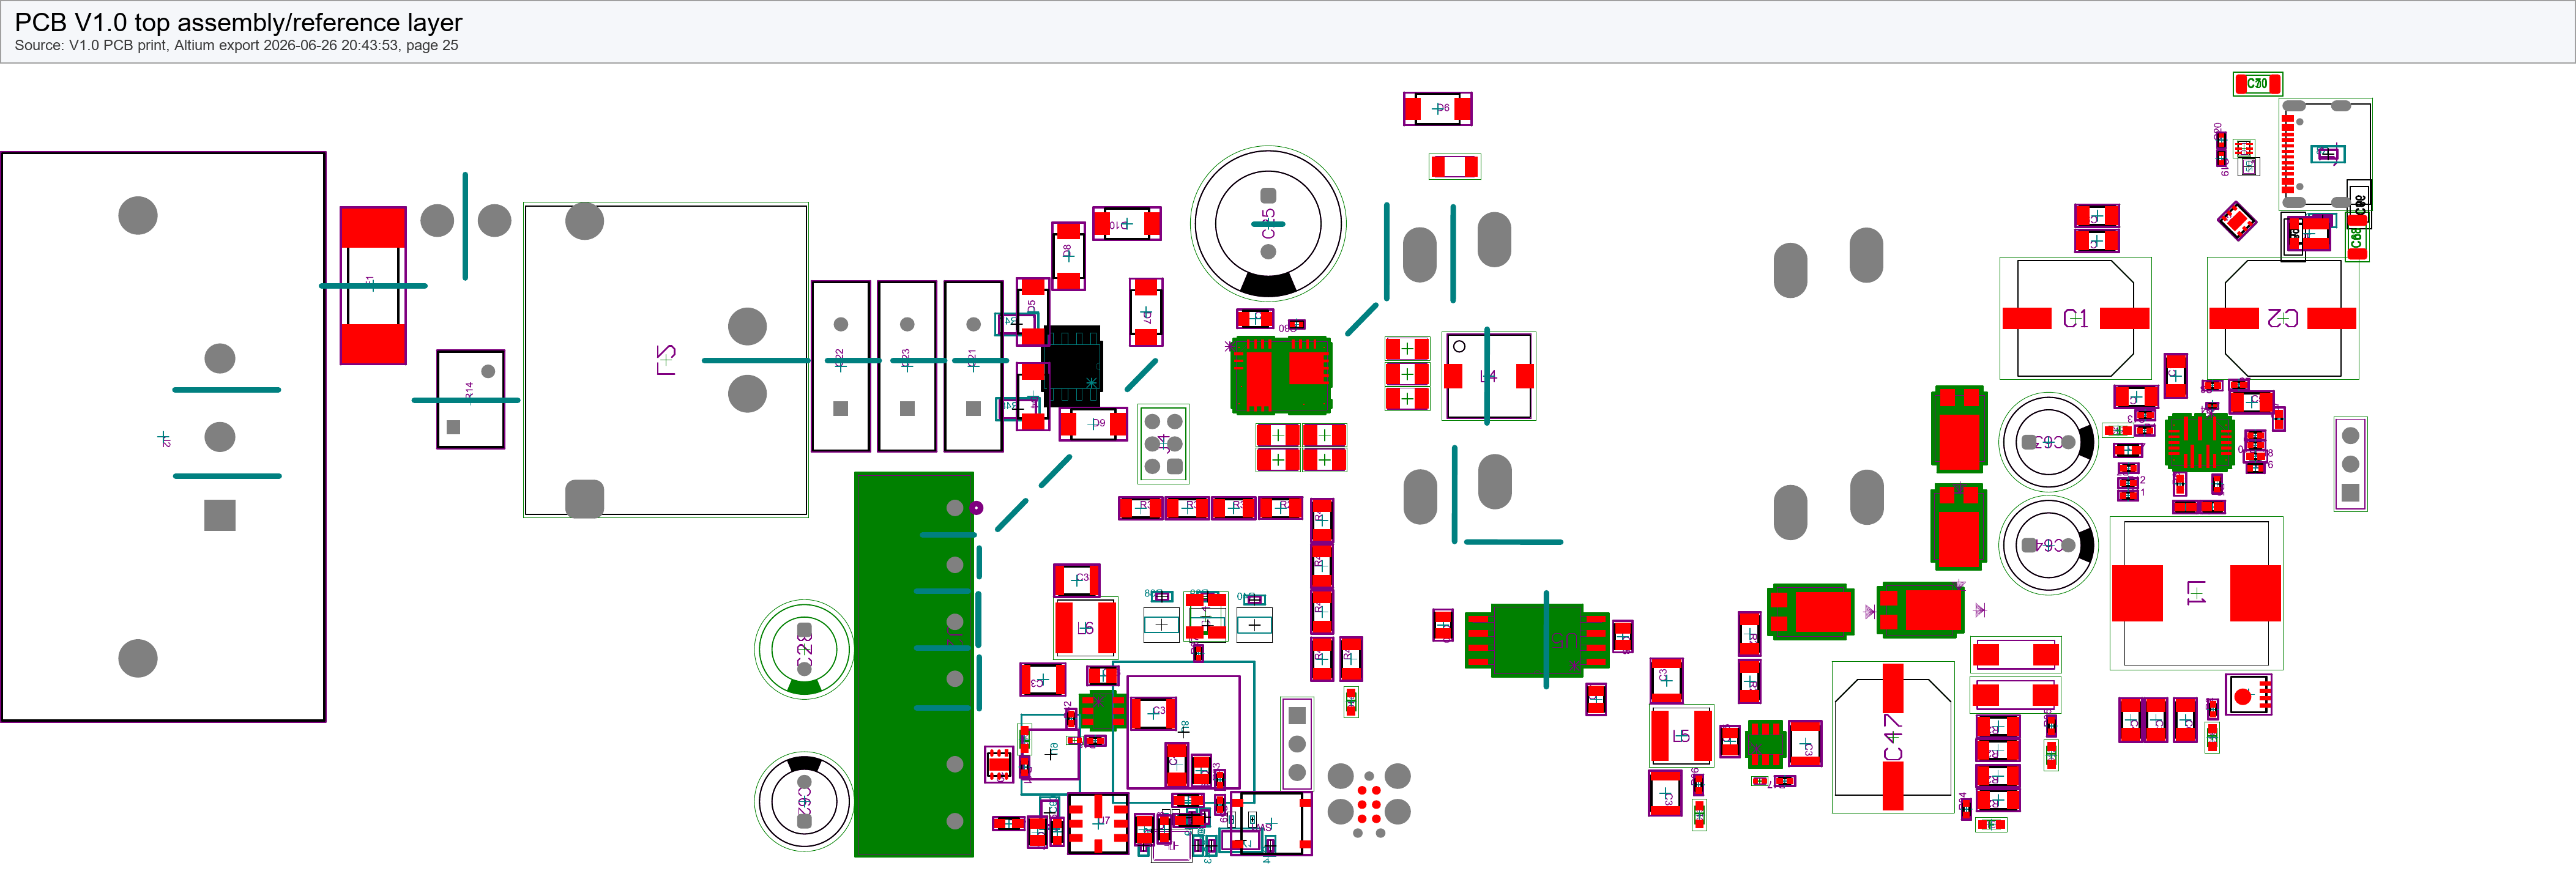
\includegraphics[width=\textwidth]{Pictures/Thesis/07_Hardware/pcb_v1_0_top_assembly_reference.png}
\caption{V1.0 top-side assembly drawing.}
\label{fig:pcb-v1-0-top-assembly-reference}
\end{figure}

\begin{table}[H]
\centering
\caption{Circuit and feedback corrections made during bring-up.}
\label{tab:hardware-implementation-lessons}
\begin{tabularx}{\textwidth}{@{}p{0.23\textwidth}X@{}}
\toprule
Item & Correction\\
\midrule
Carrier pins & PA8/PA9 form the final fixed carrier pair; PA10 provides enable. The corrected pins are shown in V1.1.\\
Charge-pump drawing & V1.1 shows the corrected diode connection and component substitutions.\\
Resonant branch & Final tests use two \SI{4.7}{\micro\henry} inductors in series.\\
PA2 feedback & The half-bridge-current signal is used for load detection; it is not the USB-C output current.\\
\bottomrule
\end{tabularx}
\end{table}

The final measurements apply to the modified V1.0 assembly and series-inductor arrangement shown here. The fitted components, calibration, and runtime settings must be reproduced along with the PCB revision.
